%EQUIVALENT RATIOS & RATIO TABLES - WORKSHEET 3
\documentclass[12pt, letterpaper, fleqn]{article}

% ----------------------------------------------------------
% PACKAGES
% ----------------------------------------------------------
\usepackage{graphicx}
\usepackage{xcolor}
\usepackage[most]{tcolorbox}
\usepackage{amsmath, amssymb}
\usepackage{fancyhdr}
\usepackage[utf8]{inputenc}
\usepackage[T1]{fontenc}
\usepackage{enumitem}
\usepackage{geometry}
\usepackage{tikz}
\usepackage{needspace}
\usepackage{multicol}

\usetikzlibrary{arrows.meta, calc}

% ----------------------------------------------------------
% PAGE SETUP
% ----------------------------------------------------------
\usepackage{times}
\geometry{letterpaper, top=1.25in, bottom=1.25in, marginpar=0.5in}

% ----------------------------------------------------------
% HEADER / FOOTER
% ----------------------------------------------------------
\newcommand{\logowidth}{3cm}
\setlength{\headheight}{20pt}
\setlength{\footskip}{40pt}

\pagestyle{fancy}
\fancyhf{}
\fancyhead[C]{\small\bfseries Equivalent Ratios \& Ratio Tables}
\fancyfoot[L]{\raisebox{2pt}{
\includegraphics[width=\logowidth]{kss.png}}}
\fancyfoot[C]{\thepage}
\fancyfoot[R]{6.3.3}

\renewcommand{\footrulewidth}{0.2pt}

% ----------------------------------------------------------
% THEME COLOR
% ----------------------------------------------------------
\definecolor{customteal}{HTML}{2fbdb9}

% ----------------------------------------------------------
% HELPER MACROS
% ----------------------------------------------------------
\newcommand{\blank}{\underline{\hspace{2.2cm}}}
\newcommand{\blanklong}{\underline{\hspace{6.5cm}}}
\newcommand{\blankshorter}{\underline{\hspace{1.5cm}}}

% ----------------------------------------------------------
% DOCUMENT
% ----------------------------------------------------------
\begin{document}


\textbf{Name:} \underline{\hspace{5cm}}
\hfill
\textbf{Date:} \underline{\hspace{3cm}}\\

% ==========================================================
% INTRODUCTION — MASTERY
% ==========================================================
\begin{tcolorbox}[colback=customteal!20]
    \large\textcolor{black}{\textbf{Mastery: Ratios, Tables, and Graphs}}
\end{tcolorbox}

\vspace{3mm}

\noindent
You now understand equivalent ratios and can create ratio tables, find missing values, and plot ratio pairs on a coordinate plane. This worksheet brings it all together!

\vspace{4mm}

% ==========================================================
% PART A — PLOTTING RATIOS ON A COORDINATE PLANE
% ==========================================================
\begin{tcolorbox}[colback=customteal!20]
\large\textcolor{black}{\textbf{Graph Ratio Tables on the Coordinate Plane}}
\end{tcolorbox}

\noindent
Complete the ratio table, then plot the points on the coordinate plane. Draw a line through the points.

\vspace{3mm}

\noindent
\textbf{1) Ratio 1:2}

\begin{center}
\begin{tabular}{|c|c|c|c|c|c|}
\hline
x & 1 & 2 & 3 & 4 & 5 \\
\hline
y & 2 & \phantom{00} & \phantom{00} & \phantom{00} & \phantom{00} \\
\hline
\end{tabular}
\end{center}

\begin{center}
\begin{tikzpicture}[scale=0.7]
\draw[gray!30] (0,0) grid (6,12);
\draw[->, thick] (-0.3,0) -- (6.5,0) node[right] {x};
\draw[->, thick] (0,-0.3) -- (0,12.5) node[above] {y};
\foreach \x in {1,2,3,4,5,6} {\draw (\x,-0.2) -- (\x,0.2) node[below=3pt] {\x};}
\foreach \y in {2,4,6,8,10} {\draw (-0.2,\y) -- (0.2,\y) node[left=3pt] {\y};}
\end{tikzpicture}
\end{center}

\newpage

\noindent
\textbf{2) Ratio 2:3}

\vspace{1cm}

\begin{center}
\begin{tabular}{|c|c|c|c|c|c|}
\hline
x & 2 & 4 & 6 & 8 & 10 \\
\hline
y & 3 & \phantom{00} & \phantom{00} & \phantom{00} & \phantom{00} \\
\hline
\end{tabular}
\end{center}

\vspace{1cm}

\begin{center}
\begin{tikzpicture}[scale=0.6]
\draw[gray!30] (0,0) grid (12,18);
\draw[->, thick] (-0.3,0) -- (12.5,0) node[right] {x};
\draw[->, thick] (0,-0.3) -- (0,18.5) node[above] {y};
\foreach \x in {2,4,6,8,10,12} {\draw (\x,-0.2) -- (\x,0.2) node[below=2pt, font=\tiny] {\x};}
\foreach \y in {3,6,9,12,15,18} {\draw (-0.2,\y) -- (0.2,\y) node[left=2pt, font=\tiny] {\y};}
\end{tikzpicture}
\end{center}

\newpage

% ==========================================================
% PART B — MULTI-STEP RATIO PROBLEMS
% ==========================================================
\begin{tcolorbox}[colback=customteal!20]
\large\textcolor{black}{\textbf{Solve Complex Ratio Problems}}
\end{tcolorbox}

\noindent
Use ratio tables to solve each problem. Show all work.

\vspace{3mm}

\begin{enumerate}[itemsep=2.3cm, leftmargin=0.6cm]

\item A school has a ratio of 3 computers to 5 students. If the school has 450 students, how many computers are there?

\begin{center}
\begin{tabular}{|c|c|c|c|c|}
\hline
Computers & 3 & & & \\
\hline
Students & 5 & & & 450 \\
\hline
\end{tabular}
\end{center}

\vspace{1.5cm}

\item A recipe calls for flour and sugar in the ratio 4:2. If you use 16 cups of flour, how much sugar do you need?

\begin{center}
\begin{tabular}{|c|c|c|c|c|}
\hline
Flour & 4 & 8 & & 16 \\
\hline
Sugar & 2 & & & \\
\hline
\end{tabular}
\end{center}

\vspace{1.5cm}

\item A car travels 150 miles in 3 hours. At this rate, how far will it travel in 8 hours?

\begin{center}
\begin{tabular}{|c|c|c|c|c|}
\hline
Miles & 150 & & & \\
\hline
Hours & 3 & & & 8 \\
\hline
\end{tabular}
\end{center}

\vspace{1.5cm}

\end{enumerate}

\newpage

% ==========================================================
% PART C — COMPARING MULTIPLE RATIOS
% ==========================================================
\begin{tcolorbox}[colback=customteal!20]
\large\textcolor{black}{\textbf{Which Deal is Better? Which is Faster?}}
\end{tcolorbox}

\noindent
Create ratio tables to compare. Circle the better option.

\vspace{3mm}

\begin{enumerate}[itemsep=2.3cm, leftmargin=0.6cm]

\item Three pizza places offer different deals:
\begin{itemize}
    \item Place A: 2 pizzas for \$16
    \item Place B: 3 pizzas for \$27
    \item Place C: 4 pizzas for \$36
\end{itemize}

Find the cost per pizza for each. Which is the best deal?

\vspace{2.5cm}

\item Two runners:
\begin{itemize}
    \item Runner 1: 15 miles in 2 hours
    \item Runner 2: 24 miles in 3 hours
\end{itemize}

Find the miles per hour for each. Who is faster?

\vspace{2.5cm}

\end{enumerate}

\newpage

% ==========================================================
% PART D — REAL-WORLD APPLICATIONS & REASONING
% ==========================================================
\begin{tcolorbox}[colback=customteal!20]
\large\textcolor{black}{\textbf{Challenge Problems}}
\end{tcolorbox}

\noindent
Solve using ratio tables. Show your complete work and explain your reasoning.

\vspace{3mm}

\begin{enumerate}[itemsep=2.5cm, leftmargin=0.6cm]

\item A painter can paint 60 square feet in 4 hours. At this rate, how long will it take to paint a 300 square foot wall?

\vspace{2.8cm}

\item A bakery makes cookies at a ratio of chocolate chip to oatmeal of 5:2. If they make 140 oatmeal cookies, how many chocolate chip cookies do they make?

\vspace{2.8cm}

\item A model train travels 1 foot for every 10 feet of real track. If the real track is 500 feet long, how long should the model track be?

\vspace{2.8cm}

\end{enumerate}


\end{document}
